%++++++++++++++++++++++++++++++++++++++++
% Don't modify this section unless you know what you're doing!
\documentclass[letterpaper,11pt]{article}
\usepackage{natbib}
\bibliographystyle{unsrtnat}
\usepackage{tabularx} % extra features for tabular environment
\usepackage{amsmath}  % improve math presentation
\usepackage{graphicx} % takes care of graphic including
\usepackage{physics}
\machinery
\usepackage{hyperref}
\usepackage[margin=1in,letterpaper]{geometry} % decreases margins
%\usepackage{cite} % takes care of citations
\usepackage[final]{hyperref} % adds hyper links inside the generated pdf file
\hypersetup{
	colorlinks=true,       % false: boxed links; true: colored links
	linkcolor=blue,        % color of internal links
	citecolor=blue,        % color of links to bibliography
	filecolor=magenta,     % color of file links
	urlcolor=blue         
}
%+++++++++++++++++++++++++++++++++++++++
\begin{document}

\title{Cource no : Qt312 and Lab No. : 1 \\\textbf{Grover algorithm}}
\author{Avinash singh}
\date{Feb 1, 2022}
\maketitle

\begin{abstract}
An unsorted database contains N records, of which just
one satisfies a particular property. The problem is to
identify that one record. Any classical algorithm, deterministic or probabilistic, will clearly take O (N) steps
since on the average it will have to examine a large fraction of the N records. Quantum mechanical systems can
do several operations simultaneously due to their wave
like properties. Therefore  O($\sqrt{N}$) step quantum mechanical algorithm for identifying that record. It
is within a constant factor of the fastest possible quantum mechanical algorithm.
\end{abstract}

\section{Introduction}

Searching large databases is an important
problem with broad applications. The Grover
search algorithm provides a powerful
method for quantum computers to perform
searches with a quadratic speedup in the number of required database queries over classical
computers. It is an optimal search algorithm for
a quantum computer , and has further applications as a subroutine for other quantum algorithms.ou have likely heard that one of the many advantages a quantum computer has over a classical computer is its superior speed searching databases. Grover's algorithm demonstrates this capability. This algorithm can speed up an unstructured search problem quadratically, but its uses extend beyond that; it can serve as a general trick or subroutine to obtain quadratic run time improvements for a variety of other algorithms. This is called the amplitude amplification trick.
\newline
\newline
The Grover search algorithm has 4 stages: \textbf {initialization}, \textbf{oracle}, \textbf{amplification}, and \textbf{measurement}. The \textbf {initialization} stage creates an equal
superposition of all states. The \textbf {oracle} stage marks the
solution(s) by flipping the sign of that state’s amplitude.
The \textbf{amplification} stage performs a reflection about the
mean, thus increasing the amplitude of the marked state.
Finally, the algorithm output is measured. For a search
database of size N, the single-shot probability of measuring the correct answer is maximized to near-unity by repeating the oracle and amplification stages O($\sqrt{N}$
) times. By comparison, a classical search algorithm will
get the correct answer after an average of N/2 queries of
the oracle. For large databases, this quadratic speed up represents a significant advantage for quantum computers

\subsection{Unstructured Search}
    Unstructured data (or unstructured information) is information that either does not have a pre-defined data model or is not organized in a pre-defined manner. Unstructured information is typically text-heavy, but may contain data such as dates, numbers, and facts as well.Suppose you are given a large list of N items. Among these items there is one item with a unique property that we wish to locate; we will call this one the winner w. Think of each item in the list as a box of a particular color. Say all items in the list are gray except the winner w, which is purple.On a quantum computer, we can find the marked item in roughly O($\sqrt{N}$ ) steps with Grover's amplitude amplification trick howerver using classical computation, one would have to check on average N/2 of these boxes, and in the worst case, all N of them
    \begin{figure}
    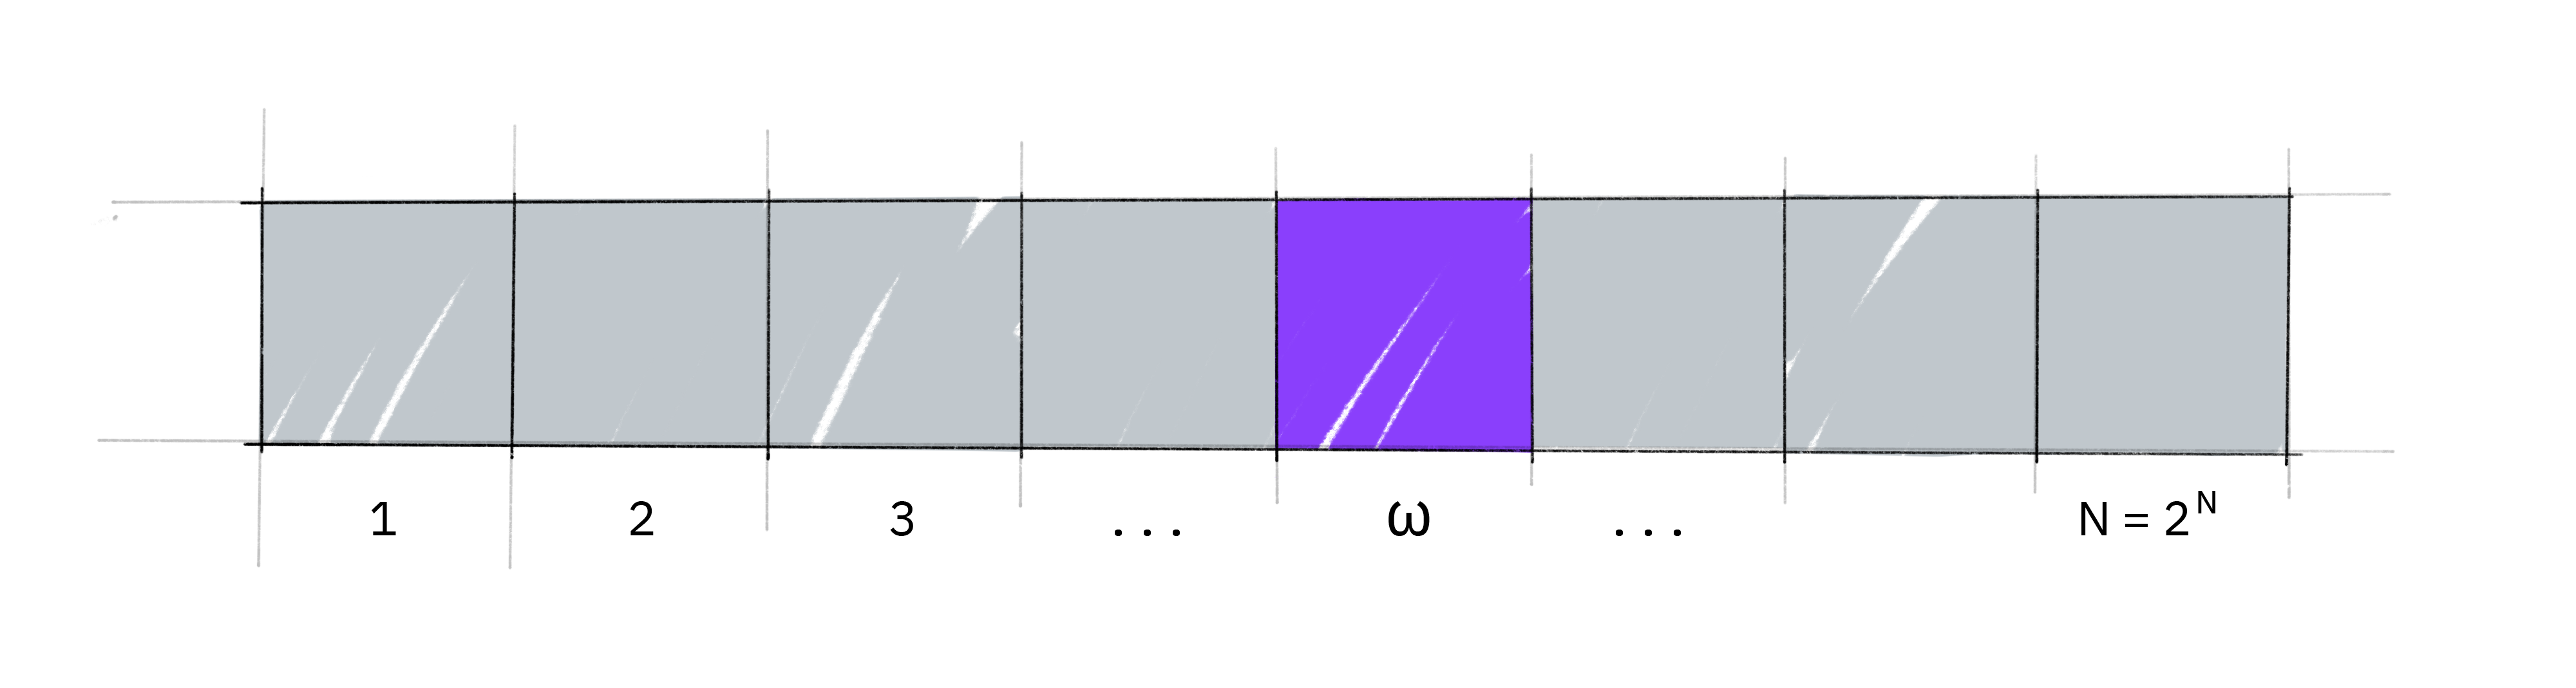
\includegraphics[width=\linewidth]{grover_list.png}
     \caption{A large list.}
    \label{fig:large list}
    \end{figure}
\subsection{The Oracle}
Suppose we are supplied with a quantum oracle with the ability to recognize
solutions to the search problem. This recognition is signalled by making use of an oracle qubit. More precisely, the oracle is a unitary operator, O, defined by its action on the
computation basic
\begin{align*}
    \ket{x} \ket{q} \rightarrow \ket{x} \ket{x \oplus f(x)}
\end{align*}
where $\ket{x}$ is the index register, $\oplus$ denotes addition modulo 2, and the oracle qubit $\ket{q}$ is
a single qubit which change sign when $\ket{x}$ is solution to search problem, initial state of $\ket{q}$ is $\frac{(\ket{0} - \ket{1})}{\sqrt{2}}$
For the examples in this textbook, our 'database' is comprised of all the possible computational basis states our qubits can be in. For example, if we have 3 qubits, our list is the states $\ket{000}$,$\ket{001}$,…$\ket{111}$ (i.e the states $\ket{0}$→$\ket{7}$)
\newline
Grover’s algorithm solves oracles that add a negative phase to the solution states. I.e. for any state $\ket{x}$ in the computational basis:
\subsection{Amplitude Amplification}
If at this point we were to measure in the standard basis {$\ket{x}$, this superposition would collapse, according to the fifth quantum law, to any one of the basis states with the same probability of $\frac{1}{N} = \frac{1}{2^n}$. Our chances of guessing the right value w is therefore 1 in 2n, as could be expected. Hence, on average we would need to try about $\frac{N}{2}$ = $2^{n-1}$ times to guess the correct item.
\newline
\newline
Enter the procedure called amplitude amplification, which is how a quantum computer significantly enhances this probability. This procedure stretches out (amplifies) the amplitude of the marked item, which shrinks the other items' amplitude, so that measuring the final state will return the right item with near-certainty.
This algorithm has a nice 2 Dimension geometry interpretation in terms of  two reflections operator. We need to consider only two-state one winner |w> state and the other is a uniform superposition $\ket{s}$ of states. These two vectors are span two-dimension plans in the herbert space of $C^N$. They are not quite perpendicular to each other because $\ket{w}$ is occur in a superposition of $\ket{s} $with an amplitude of $N^\frac{-1}{2}$ as well. Now take another state $\ket{s’}$ which is perpendicular to the state  $\ket{w}$. This obtained from $\ket{s’}$ by removing the state $\ket{w}$ from it.
\newline
\newline
$\small\textbf{STEP 1:}$ 
The amplitude amplification procedure starts out in the uniform superposition $\ket{s}$, which is easily constructed from $\ket{s} = H^{\oplus n}\ket{0}^n$.

\begin{figure}[h!]
    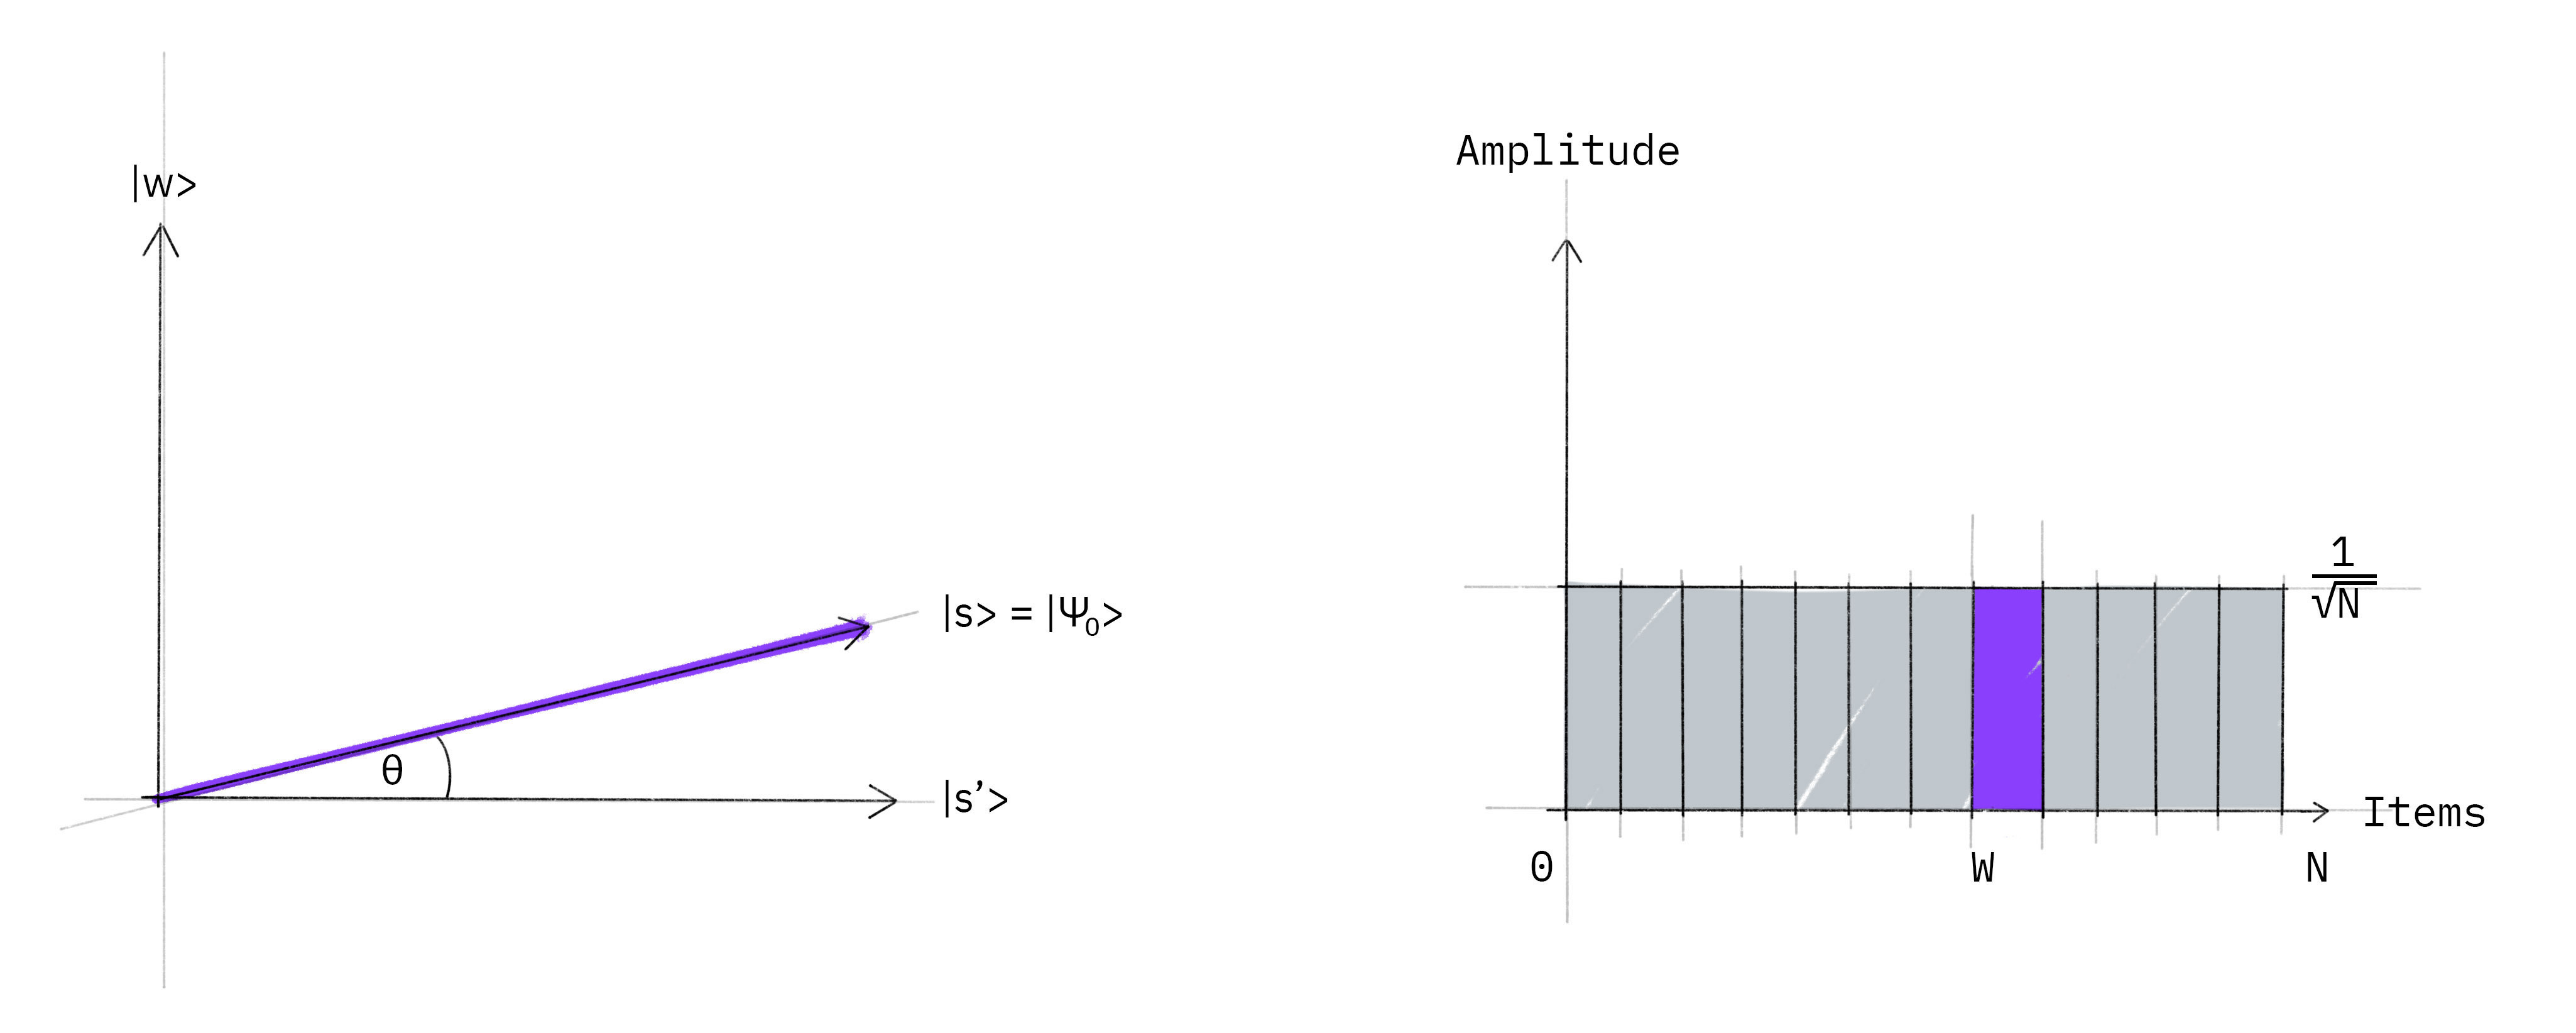
\includegraphics[width=\linewidth]{grover_step1.jpg}
\end{figure}

\newline 
$\small\textbf{STEP 2:}$  We apply the oracle reflection $U_f$ to the state $\ket {s}$.

\begin{figure}[h!]
    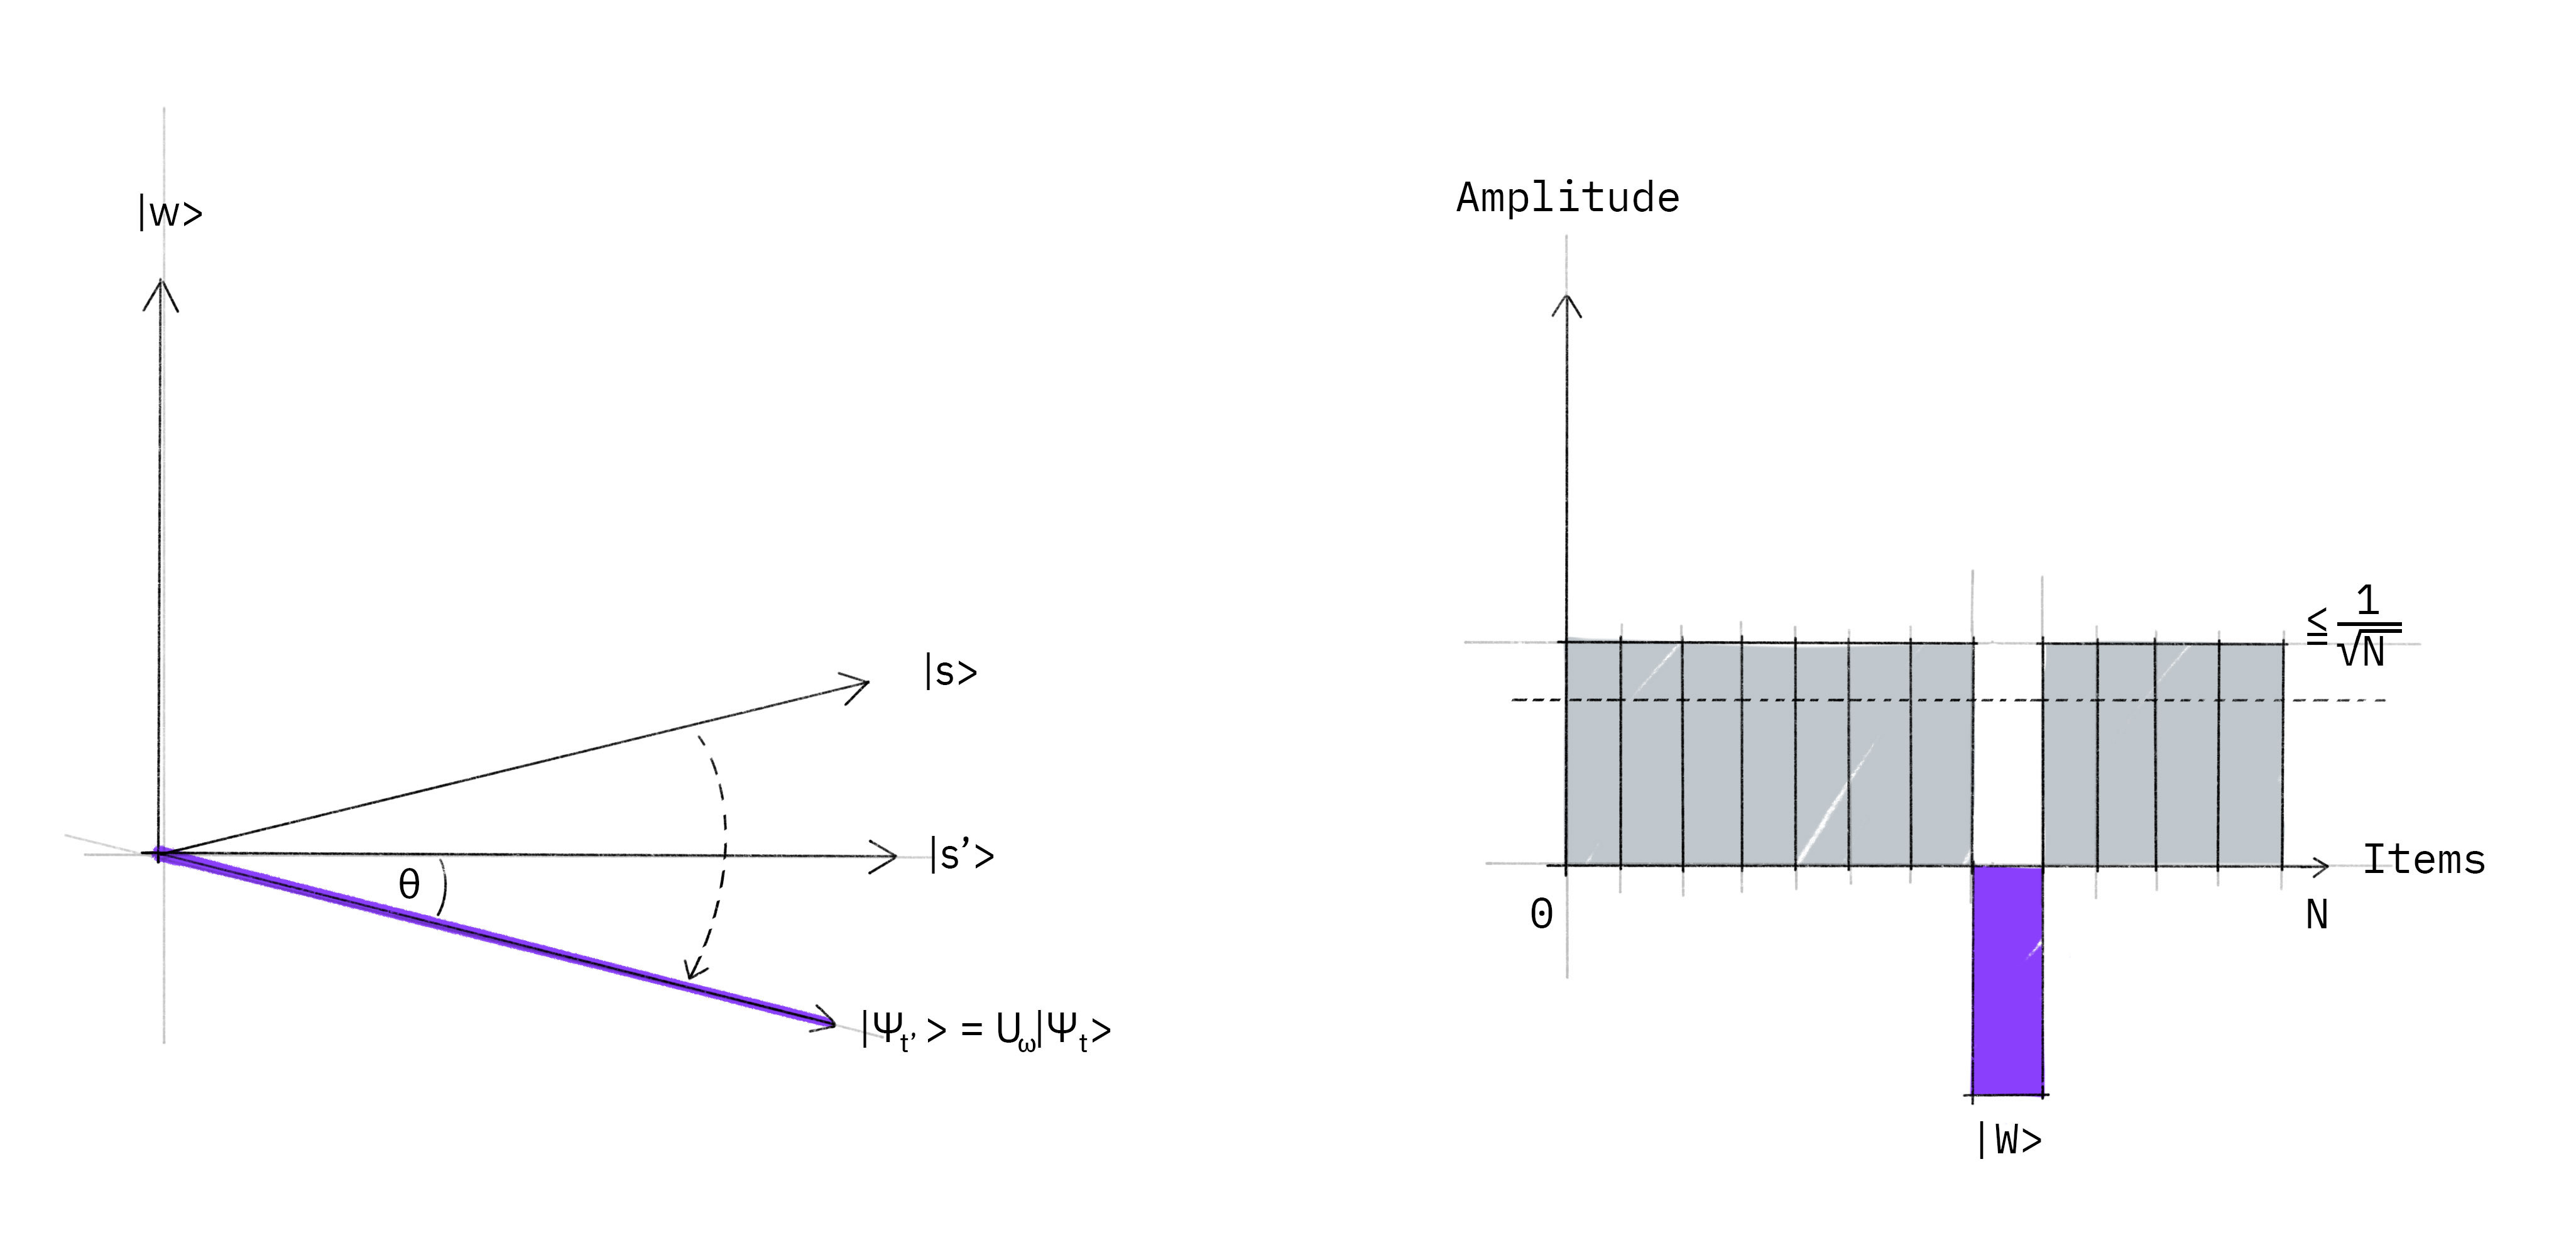
\includegraphics[width=\linewidth]{grover_step2.jpg}
\end{figure}
$\small\textbf{STEP 3:}$
We now apply an additional reflection $U_s$ about the state $\ket{s}$: $U_s = 2\ket{s}\bra{s} - 1$.This transformation maps the state to $U_s U_f \ket{s}$ and completes the transformation.
\begin{figure}[h!]
    \centering
    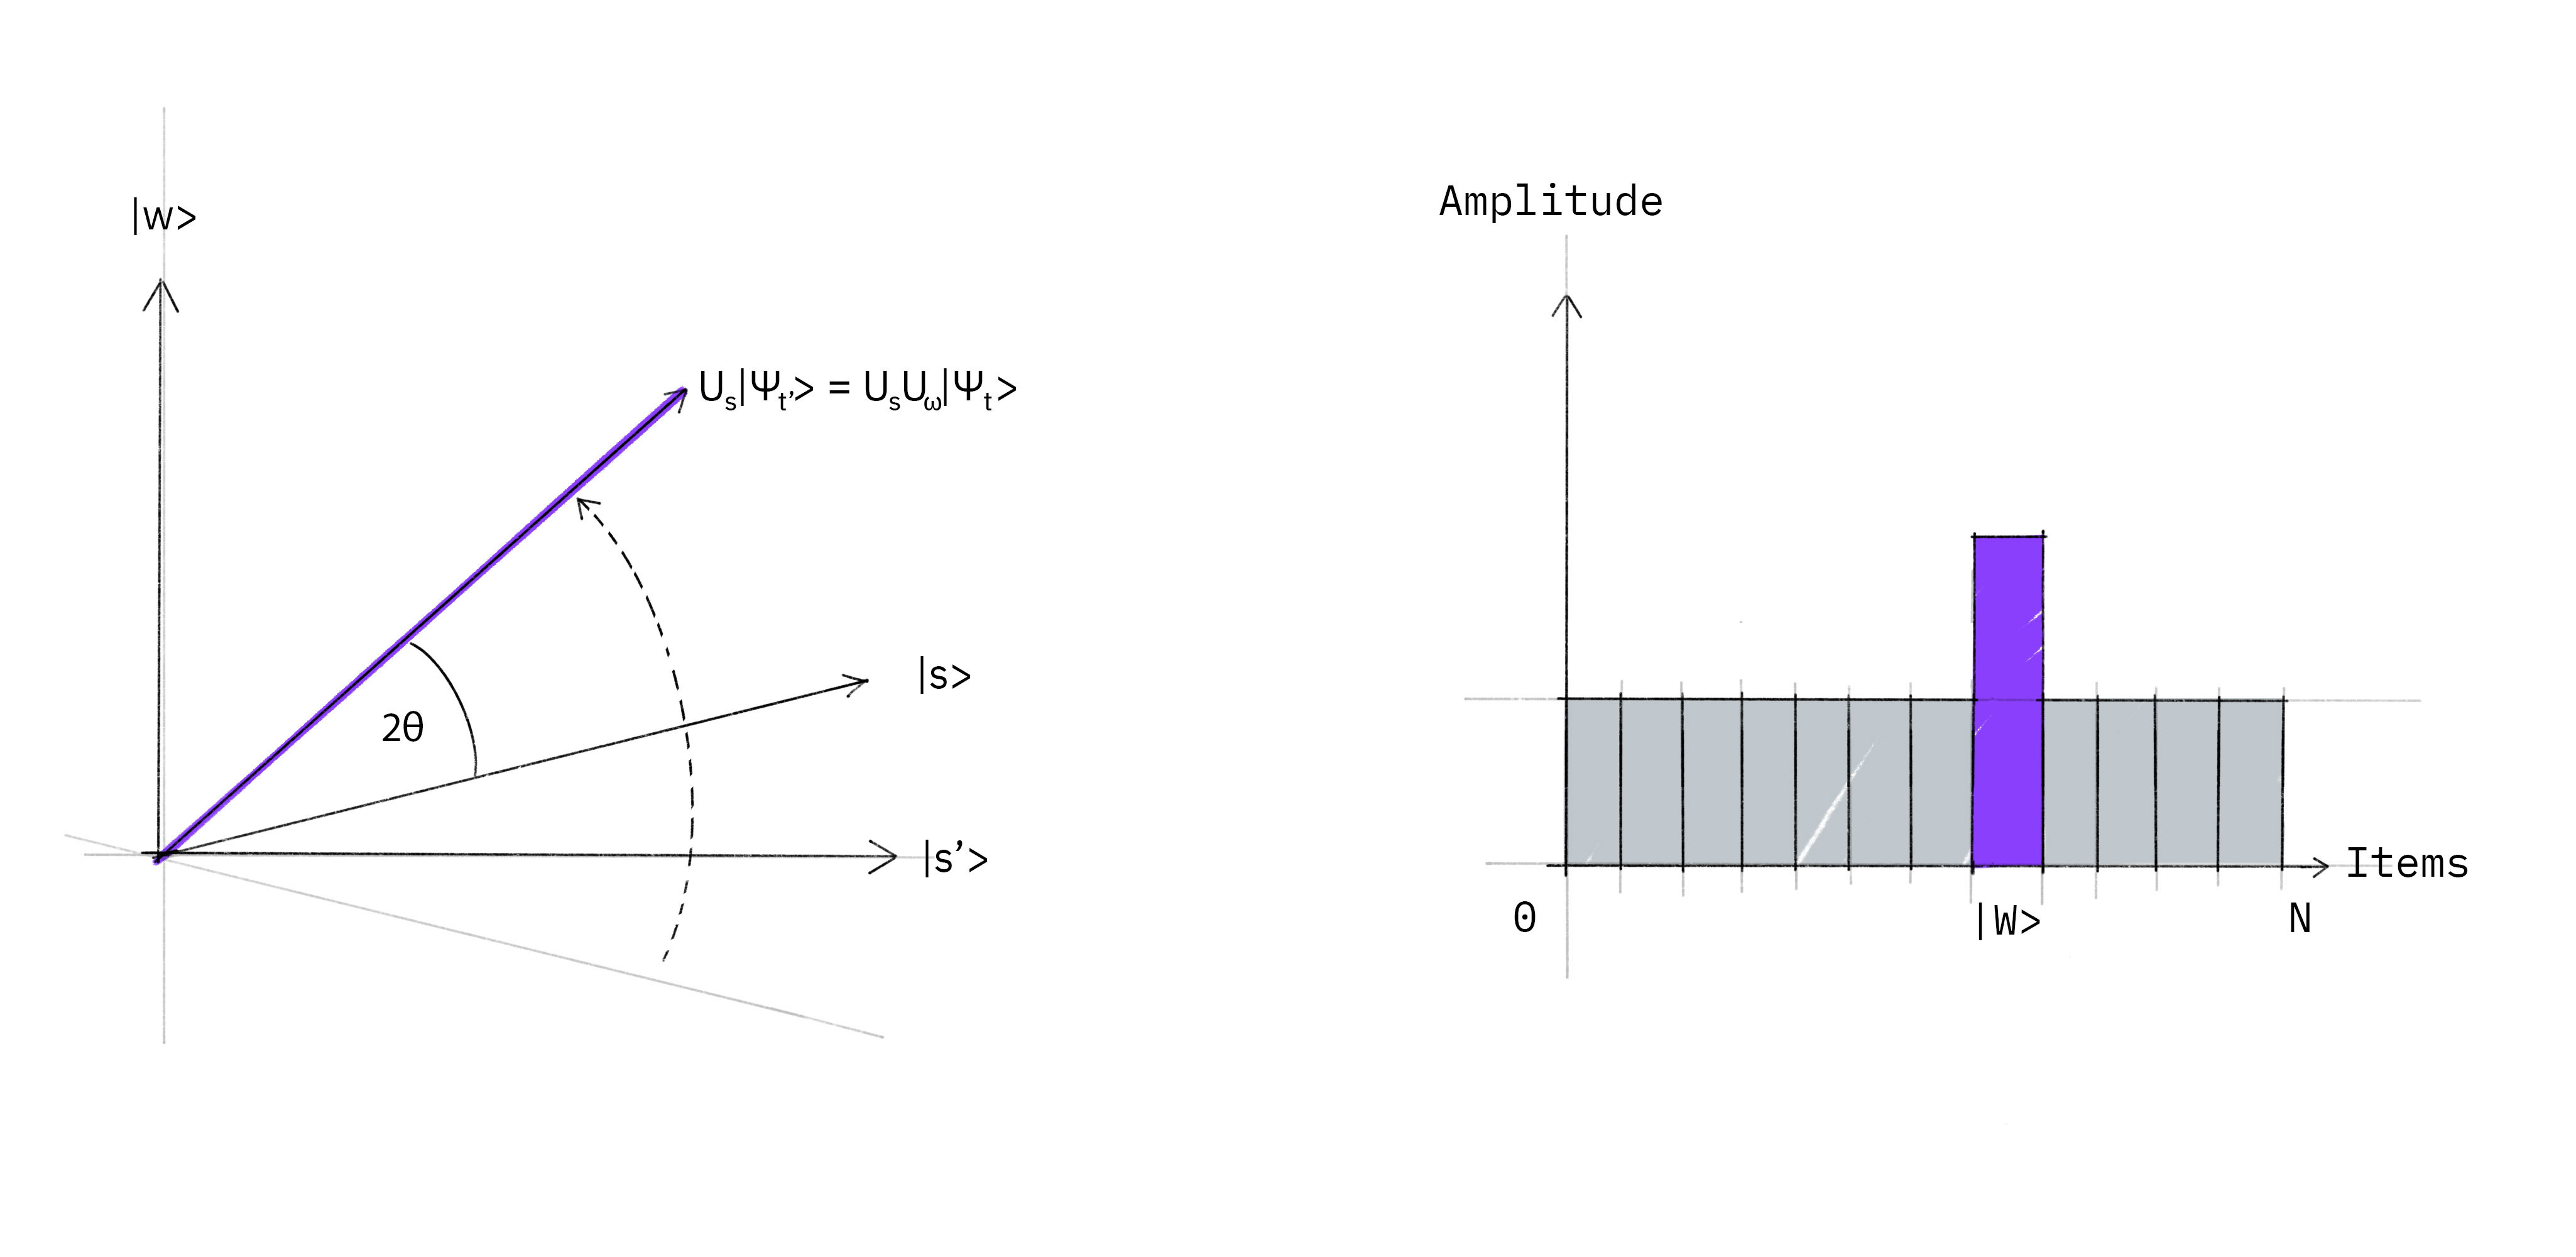
\includegraphics[width=\linewidth]{grover_step3.jpg}
\end{figure}
\par 
Two reflections always correspond to a rotation. The transformation UsUf rotates the initial state |s⟩ closer towards the winner |w⟩. The action of the reflection Us in the amplitude bar diagram can be understood as a reflection about the average amplitude. Since the average amplitude has been lowered by the first reflection, this transformation boosts the negative amplitude of |w⟩ to roughly three times its original value, while it decreases the other amplitudes. We then go to step 2 to repeat the application. This procedure will be repeated several times to zero in on the winner.
\newline
After t steps we will be in the state  	$\ket{\psi_t}$ where: $\ket{\psi_t} =(\ket{U_s}\ket{U_f})^t\ket{s}$.
\newline
\begin{figure}[h!]
    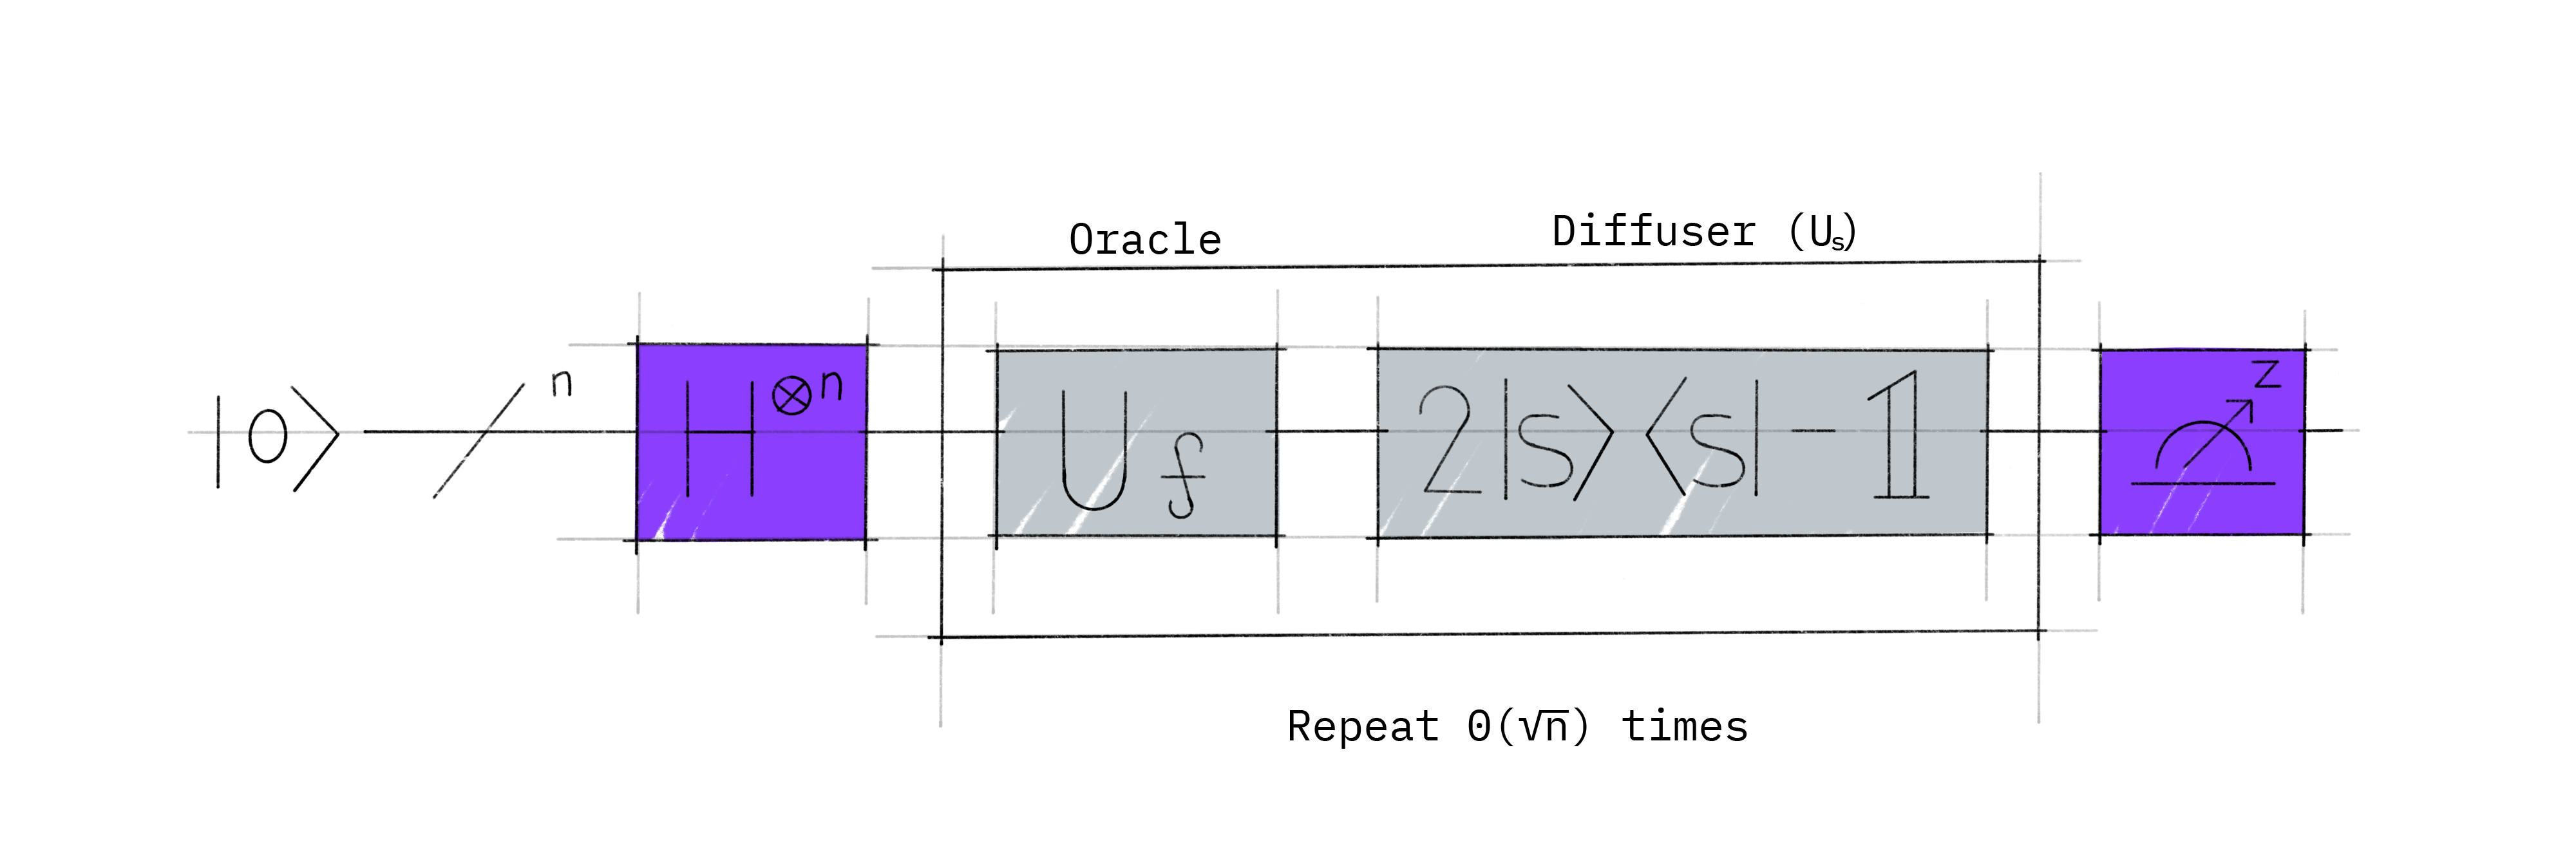
\includegraphics[width=\linewidth]{grover_circuit_high_level.png}
     \caption{Full grovers circuit.}
    \label{fig:Full grover circuit.}
    \end{figure}
\newline
After repeating this operation $\sqrt{N}$ we get get winner state will emerge out. If we left for long time Then the probability of finding operator is a decrease 
\subsection{Result}
Then the probability of finding operator is a decrease 
I have Implemented a Grover circuit with a database for 3 qubits it gives a result with an accuracy of around 80$\%$ and for the real device (ibm-lagos) its accuracy comes down to 40 $\%$. This error is coming due to large circuit formation, which introduces an error in the result. After transpiling the circuit, we can see the size circuit which is big. I putting githublink for notebook.
\newline
This is my link for: \href{https://github.com/AvinashQtC/Quantum_Algo/blob/main/grover1.ipynb}{Jupyter Notebook}.

\end{document}
